

\DeclarePairedDelimiter{\norm}{\lVert}{\rVert}



\newcommand{\sumn}[1]{\sum\limits_{{#1}=1}^{n}}
\newcommand{\derivative}[2]{\dfrac{\partial {#1}}{\partial {#2}}}
%\newcommand{\subsubsubsection}[1]{\paragraph{#1}\mbox{}\\}

\newcommand{\subsubsubsection}[1]{ \noindent \textbf{#1} }




% Ajánlott minden fő fejezetet külön fájlba írni, pl.:



%\include{tex/bevezeto}
%\include{tex/felhasznaloi}
%\include{tex/fejlesztoi}
%\include{tex/irodalom}



%A diplomamunkának a következő fő részekből kell állnia: 
%1. A dolgozatban megoldott probléma megfogalmazása.
%2. A problémakör irodalmának, az előzményeknek rövid áttekintése.
%3. A probléma megoldásának részletes ismertetése, a választott megoldás indoklása.
%4. Az eredmények összefoglaló értékelése és a levonható következtetések leírása.
%5. 5. Ha a diplomamunka fő eredménye egy program, akkor a dolgozat része a program felhasználói
%dokumentációja, fejlesztési dokumentációja

% III. A diplomamunkára vonatkozó formai követelmények:
% 1. A diplomamunkát nyomtatva, bekötve kell benyújtani az illetékes tanszékre.
% 2. A diplomamunka első oldalán fel kell tüntetni a diplomamunka címét, szerzőjének nevét,
% szakját, az illetékes tanszéket, a témavezető nevét, a külső konzulens nevét, a beadás helyét és
% a védés évét.
% 3. A dolgozat 2. oldala a hivatalos diplomamunkai témabejelentő.
% 4. A Bevezetés tartalmazzon a Diplomamunka-téma bejelentő lapon kitűzött feladat teljesítésének
% mértékére vonatkozó információt.
% 5. A diplomamunka fő részei a dolgozat önálló fejezetei legyenek.
% 6. A diplomamunkának legyen Tartalomjegyzéke és a felhasznált irodalomról Irodalomjegyzéke.
% 7. A diplomamunkában be kell tartani a hivatkozások és idézések standard szabályait. 

\section{Bevezetés}

Amióta csak az ember fizetőeszközöket használ jelen volt párhuzamosan a hamisítás is.
Ezért mindig is igény volt arra, hogy mikor a javak gazdát cseréltek a felek meg tudjanak 
bizonyosodni a valuta érvényességéről. Amíg aranypénzt használtak gondoljuk csak arra, hogy
annak puhaságát kihasználva az emberek ráharaptak, hogy ezzel is ellenőrizzék. Hasonló példa 
mikor Arkhimédész egy aranykorona sűrűségét mérte meg, ezzel megállapítva, hogy az részben ezüst
volt. Látható, hogy az aranyat nem volt egyszerű hamisítani, de a hordozása nagyobb 
mennyiségben bajos volt, könnyen eshetett az ember rablók áldozatául.

Mikor ennek kivédésére a bankok papírpénzt kezdtek kibocsátani, ez a probléma némileg orvosolódott,
de újakat vetett fel: megjelentek a hamisítók, akik ezzel akartak könnyen vagyonhoz jutni.
Ezért onnantól kezdve, egészen a mai napig a bankjegynyomdák feladata, hogy olyan
technológiát használjanak, ami egy egyszerű ember számára drága vagy egyáltalán nem elérhető,
ezáltal nem reprodukálható.

Eleinte elég volt, hogy mikor a bank aranyra váltotta a készpénzt, akkor az ottani szakképzett
alkalmazott fel tudja ismerni a hamisítványt, de idővel felmerült az igény, hogy az utca embere
is képes legyen erre.

Ezért a nyomdák elkezdtek olyan elemeket tenni a bankjegyekre, amelyek könnyen felismerhetőek,
például vízjel, vagy színváltó tinta. Ezek jellemzője, hogy bármennyire hatásosak, drágák.
Bár a pénznyomtatásban általában rendelkezésre áll az anyagi háttér, nem ők az egyetlen
célközönség, léteznek kisebb védelmet igénylő nyomatok is, gondoljuk például egy 
zárjegyre vagy egy BKV jegyre.

Szeretnénk tehát egy olyan védelmet, amit bárki ellenőrizni tud, mégis olcsó. Erre egy megoldás,
hogy a nyomatban elhelyezett mintát egy okostelefonra készült alkalmazással lefényképezzük,
elemezzük, és ez alapján eldöntjük, hogy az eredeti-e.


Egy ilyen megoldást készített a Jura Trade kft. is. Ezen dolgozat célja ennek az alkalmazásnak
a továbbfejlesztése gépi tanulással: \textit{Támasztóvektor Gépekkel} és \textit{Konvolúciós Hálókkal},
melyek napjainkban egyre nagyobb szerepet kapnak az informatika számos területén, ebben a 
témakörben mégsem alkalmazta őket egyelőre senki.

A dolgozat első felében bemutatunk egy módszert, amivel automatizálni lehet egy döntési folyamatot, már 
meglévő, determinisztikusan előállított adatok alapján. A második részben megkísérlünk építeni egy 
önálló alkalmazást, amely semmilyen korábban megírt programra vagy algoritmusra 
nem támaszkodik, hanem a nyers képekből próbál meg egy mély neuronhálót betanítani, 
amely ezután magában alkalmas eredetiség-ellenőrzésre.


%
%ókor : arany
%-> fel tudta bárki ismerni -> ld ráharapás, sűrűség mérés.
%modern technológia -> arany nem viable
%papírpénz -> elérhető a technológia földi halandóknak
%-> egyre jobb hamisitványok -> fejlődnia kell a felismerésnek is
%aktív+passzív védelem
%minden féle cuccot ráraknak, nehéz egyszerre mindent 
%csináltak olyat is ami lerí, és olyan ami uv lámpa
%olcsó is legyen -> pénznél van pénz -> nem csak pénz

\newpage
\section{Háttér}

%
%
%TODO
%nyomdász
%vonalvastagság
%legkisebb nyomtatható elem
%különböző nyomda és fénymásoló technika
%akár azt is meg lehet mondani mivel készült
%aktív track and trace + biztonsági elemek
%-> másfeles kategóriás cuccot szeretnénk
%OVD




\subsection{Mikor biztonságos egy nyomat?}

Alapvetően akkor, hogy ha megpróbáljuk valahogy reprodukálni, akkor
mérhető lesz a különbség az eredeti és a hamis között.

Ha védeni szeretnénk egy dokumentumot vagy bankjegyet általában 
többféle módszert használunk egyszerre, amelyek optimális esetben 
ortogonálisak, tehát hamisításnál mindegyikre valahogy máshogyan kell 
felkészülni. Ezek a \textit{feature-öket} alapvetően két kategóriába tudjuk sorolni. 
Az első amit az utca embere is könnyen ellenőrizhet, például a Magyar Forintokon 
a fémszalag, vagy a színváltó tinta, de akár a papír taktilitása is.
A második amihez már valamilyen speciális eszköz is kell. Erre a legismertebb 
példa az UV lámpa, ami mindenhol megtalálható ahol pénz forog.
A valóságban létezik egy harmadik kategória is, ami a titkos, csak 
laborban kimutatható tulajdonságokat tartalmazza, de ezekkel érthető
módon nem foglalkozunk.


\subsection{Előző megoldások}

Ha egy nyomdász vagy szakértő ránéz egy biztonsági nyomatra, 
általában már a hagyományos, tintával készült részekből meg tudja
állapítani az eredetiséget. Ennek oka, hogy a hamisításhoz jó esetben nem áll 
rendelkezésre sem ugyanolyan papír, sem ugyanolyan nyomtató vagy olyan fénymásoló,
amely pont olyan eredményt produkál mint az eredeti.
Ennek feltétele, hogy mikor tervezzük a nyomatot tudjuk azt, hogy
milyen géppel fog készülni, és úgy tervezzük meg a nyomtatandó struktúrákat,
hogy azok éppen csak nyomtathatóak legyenek.


Kézenfekvő, hogy ezt a tudást szerették volna algoritmizálni. Így születtek olyan
programok amik ilyen képek alapján próbálják megállapítani az eredetiséget. 
Ilyenkor készítettek különböző hamisítványokat, és összehasonlították őket az eredetiekkel,
és addig csiszolták az algoritmusokat, amíg azok elfogadható eredményeket nem adtak.


Így születtek olyan megoldások, amik az első és a második fent említett kategória 
közé esnek, azaz az utca emberének lettek tervezve, de mégis céleszközt használva
ellenőrzik a nyomatot, ám ezeket egy okostelefon birtokában bárki elérheti.
Az ötlet, hogy lefényképezzük a dokumentumot, és ezt helyben, egy \textit{appal} elemezzük.


Speciálisan, az általunk részben felhasznált megoldás különböző szempontok alapján méréseket
végez a képen, és néhány (nagyságrendileg 10-12) mérőszámot ad eredményül, melyeket aztán
aggregál, és egy döntést hoz: \textit{Eredeti, Hamis, Nem tudjuk eldönteni bizonyosan}.

A \textit{Nem tudjuk} esetet több dolog is kiválthatja, például nagyon jó hamisítvány is,
de akár egy rossz kép is, például ha remegett az ember keze fényképezéskor.

\subsection{Gépi tanulás}

%TODO valamit általánosan a gép tanulásról?

Gépi tanulásról beszélünk, mikor egy modellt nem programozással alakítunk, hanem példákat 
mutatunk neki, és azokat egy tanulóalgoritmus beépíti a rendszerbe, ideális esetben úgy,
hogy a rendszer teljes hatékonysága javuljon. 

Manapság egyre több területen használják, például mintafelismerésre: gyógyászat, önvezető autók, nyomtatott szöveg felismerése, klaszterezésre: adatbányászat, szociális hálók vagy 
például mesterséges intelligenciák készítésére: ajánló rendszerek, csevegő robotok, játékok (például Go vagy Sakk).

Alapvetően két nagy csoportja létezik: felügyeletlen és felügyelt tanulás.
Előbbihez nem áll rendelkezésünkre általános igazság (\textit{ground truth}), nem
tudjuk mit szeretnénk megtanítani, az cél hogy a modell magától találjon új összefüggéseket.
Mi a második témakörrel foglalkozunk: rendelkezésre állnak a tanító példák és a hozzájuk
tartozó elvárt kimenetek. Ezen belül is a Támasztóvektor Gépeket és a Mély Konvolúciós hálókat
fogjuk alkalmazni.


\subsubsection{Támasztóvektor Gép}

A Támasztóvektor Gép (Support Vector Machine, SVM) egy klaszterező eljárás, amivel egy adathalmaz két csoportra bontható. 

Alapja, hogy teret egy hipersíkkal ketté osztjuk úgy, hogy a két csoport előjeles távolsága ($ d_1, d_2 $) a hipersíktól maximális legyen. 
Egy csoport és sík távolsága alatt a sík és az ahhoz legközelebbi, az adott csoportba tartozó elem távolságát értjük. 


A két távolság összegét hívjuk \textit{margónak}: $ d = d_1 + d_2 $.

A bemenő adatok vektorait $ \underline{x_i} $-vel, a hozzájuk tartozó kimenetet
$ y_i $-vel, ahol $ y_i=-1 $, ha az első csoportba tartozik, és $ y_i=1 $, ha a másodikba.

A hipersíkot a normálvektorával(súlyával, weight): $ \underline{w} $, és \textit{bias}-szal 
(részlehajlás): $ b $ ábrázoljuk.


Ekkor a sík pontjai $ \underline{x}: \underline{x}^T \cdot \underline{w} - b = 0 $

A csoportok margójához tartozó hipersíkok pedig:

$ \underline{x}: \underline{x}^T \cdot \underline{w} - b = +1 $

$ \underline{x}: \underline{x}^T \cdot \underline{w} - b = -1 $
\\
Ekkor a feladat $ \underline{w} $ és $ b $ meghatározása úgy, hogy 

$ \underline{x}^T \cdot \underline{w} - b \geq +1 $ ha $  y=1 $

$ \underline{x}^T \cdot \underline{w} - b \leq -1 $ ha $  y=-1 $

Ekkor $ d_1 = d_2 = \frac{2}{\norm{\underline{w}}} $  
\\
Mivel $ d $-t szeretnénk maximalizálni, a feladat felírható:

$ y_i \cdot (\underline{x}^T \cdot \underline{w} + b) \geq 1 $

$ \min\limits_{w, b} \norm{\underline{w}} $

Ez azonban csak akkor működik, ha az adat lineárisan szeparálható. Ellenkező esetben
vezessünk be egy olyan költségfüggvényt, ami azt bünteti ami rossz oldalon van.

$ J(\underline{w},b)  = \frac{1}{n} \sum\limits_{i=1}^{n} 
max(0, 1 - y_i(\underline{w} \cdot \underline{x} - b) + \lambda \norm{\underline{w}} $



\noindent
Megmutatható, hogy a feladat megegyezik a következővel (duális probléma): 

$ \max\limits_{c_1 \dots c_n} \sum\limits_{i=1}^{n}c_i -  $
$ \frac{1}{2}\sumn{i}\sumn{j} y_i c_i (x_i \cdot x_j) y_i c_j $

\noindent
ahol $ \forall i: $

$  \sumn{i} c_i y_i = 0 $

$ 0 \leq c_i \leq \frac{1}{2n\lambda} $

\noindent
Ennek megoldására létezik hatékony numerikus módszer.

\noindent
Ekkor a súlyok:

$ \underline{w} = \sumn{i} c_i y_i x_i $

\noindent
Keressünk egy margón lévő $ (x_i, y_i) $ párt:
$ b = \underline{w}^T \cdot \underline{x}_i  - y_i$

\noindent
Egy minta osztályozása:

$ \overline{y} = sgn(\underline{w} \cdot \underline{x} - b) $

\noindent
TODO mennyire részletezzem, hogy ezt hogy kell megoldani?




%\paragraph{Nem lineáris feladatok} 
\subsubsubsection{Nem lineáris feladatok} 


Sok esetben a feladat nem lineárisan szeparálható, viszont ha a problémateret
transzformáljuk, lehet hogy már igen. 

Vezessük be a bázisfüggvényeket, amelyek az eredeti adatot egy másik térbe,
a jellemző(\textit{feature}) térbe képezik:


$ \varphi : \mathbb{R}^n \rightarrow \mathbb{R}^m $

(általában $ m >> n $ )


\noindent
Ekkor a feladat a következőképpen módosul:

$ \max\limits_{c_1 \dots c_n} \sum\limits_{i=1}^{n}c_i -  $
$ \frac{1}{2}\sumn{i}\sumn{j} y_i c_i (\varphi(x_i) \cdot \varphi(x_j)) y_i c_j $

\noindent
ahol $ \forall i: $

$  \sumn{i} c_i y_i = 0 $

$ 0 \leq c_i \leq \frac{1}{2n\lambda} $

\noindent
és ekkor

$ \underline{w} = \sumn{i} c_i y_i \varphi(x_i) $

\noindent
Keressünk egy margón lévő $ (x_i, y_i) $ párt:

$ b = \underline{w}^T \cdot \varphi(\underline{x}_i)  - y_i$


\noindent
Egy minta osztályozása ekkor:

$ \overline{y} = sgn(\underline{w} \cdot \varphi(\underline{x}) - b) $


\paragraph{Kernel trükk} 

A jellemzőtér nagy, vagy akár végtelen dimenziós is lehet. Bizonyos esetekben a fenti képletben lévő
$ \varphi(x_i) \cdot \varphi(x_j) $ skaláris szorzatot ki tudjuk számolni anélkül, hogy a transzformációt 
elvégeznénk.



\noindent
Ehhez vezessük be a \textit{kernel függvényeket}:

$ K(x_i, x_j) = \varphi(x_i)^T \cdot \varphi(x_j) $

\noindent
Látható, hogy a maximalizálás ekkor is elvégezhető:


$ \max\limits_{c_1 \dots c_n} \sum\limits_{i=1}^{n}c_i -  $
$ \frac{1}{2}\sumn{i}\sumn{j} y_i c_i k(x_i, x_j) y_i c_j $

\noindent
ahol $ \forall i: $

$  \sumn{i} c_i y_i = 0 $

$ 0 \leq c_i \leq \frac{1}{2n\lambda} $

\noindent
És a predikció is csak kicsit módosul
egy $ x' $ mintára:

$ y' = sgn(\underline{w} \cdot \varphi(\underline{x}) - b) = $
$ sgn(\sumn{i} c_i y_i k(\underline{x}_i, \underline{x}') - b) $


%TODO mutassunk bázisfüggvényeket
%ez a megvalósítás részbe került
% de az rbf ez lehet hogy ide lehetn rakni?...


\subsubsection{Mély hálók}

Általánosságban egy mély háló egy nagy bemenetet (ez esetben képet) úgy képez
a kimenetre, hogy több kisebb lépésben tömöríti az inputot rejtett rétegek segítségével,
amíg a dimenziója el nem éri a várt kimenetét. 
(Nálunk ez egy 0 és 1 közti szám, ahol 1 az eredeti, 0 a hamis.)


Ez egy felügyelt tanulás, tehát a háló tanításához szükségünk van az inputhoz ($ \underline{x} $) 
tartozó outputra, a \textit{ground truth}ra ($ \underline{y} $). 
A háló súlyait kezdetben véletlenszerűen inicializáljuk.
Ezután minden iterációban néhány inputra lefuttatjuk a hálót, 
kapva ezzel egy kimenetet ($ \underline{y}' $).

\noindent
Nézzük ekkor a négyzetes hibát($ J $) a belső súlyok függvényében($ \underline{w} $):

$ J(\underline{w}) = \sumn{i} \norm{y_i-y_i'}_2^2 $

\noindent
Bár többféle algoritmus létezik, lényegében mindegyik ennek a hibafüggvénynek
a minimalizálására törekszik, és általában a Gradiens módszeren alapulnak.
A különbség a konvergencia sebessége és a lokális szélsőértékkel szembeni 
hibatűrő képességükben van.

Ehhez visszafelé haladva (\textit{backpropagation}) rétegenként visszaterjeszti a hibát,
és a gradienssel ellentétes irányba $ \underline{w} $-t, így csökkentve a költségfüggvény értékét.


$ \underline{w}' = \underline{w} - \gamma \cdot \triangledown J(\underline{w})$

\noindent
Ahol $ \gamma < 1 $ a tanulási együttható.


\noindent
\paragraph{Példa}
Tekintsünk egy sűrű perceptron réteget, ahol $ (x_i, y_i) $ a 
bemenet és a hozzá tartozó kimenet:

$ \underline{y}' = Relu(W \cdot \underline{x} + \underline{b}) $

$ W' = W - \gamma \cdot  \triangledown  J(\underline{W})$
$ = W - \gamma \cdot \derivative{J(W)}{W} $

$ = W - \gamma \cdot  \derivative{ \dfrac{1}{n} \sumn{i} \norm{y_i-y_i'}_2^2}{W} $


$ = W - \gamma \cdot \derivative{ \dfrac{1}{n} \sumn{i} \norm{y_i-Relu(W \cdot \underline{x}_i + \underline{b})}_2^2}{W} $

$ = W - \gamma \cdot \dfrac{1}{n} \sumn{i} 2 (y_i-Relu(W \cdot \underline{x}_i + \underline{b})) \cdot   $
$ Relu'(W \cdot \underline{x}_i + b) \cdot  diag(\underline{x}_i) $


\noindent
ahol Relu - \textit{Rectified Linear Unit}:


$ Relu(x) =  $
$ \begin{cases}
x, & \text{ha}\ x > 0 \\
0, & \text{különben}
\end{cases} $

$ Relu'(x) =  $
$ \begin{cases}
1, & \text{ha}\ x > 0 \\
0, & \text{különben}
\end{cases} $

$ Relu(\underline{x}) = (Relu(x_1), Relu(x_2) \cdots Relu(x_n))^T $



\subsubsection{Rétegek}


Egy mély háló különböző rétegekből épülhet fel, ám a fenti deriváltakat
mindig ki lehet számolni analitikusan, ezzel növelve a robosztusságot.
Nézzük mi milyen rétegeket használunk!

\paragraph{Sűrű} (\textit{dense}) rétegről beszélünk, ha a bemenet és kimenet 
minden pontja között van kapcsolat.

\paragraph{Aktivációs} réteg például a fenti $ Relu() $ függvény, ami 
valamilyen nem-linearitást visz a modellbe, ezáltal növelve a háló 
kifejezőerejét. Ha ez nem lenne $ W_1 \cdot W_2 \cdot W_3 $ a szorzást 
elvégezve összevonható lenne egy közös $ W $ mátrixba, tehát redundáns 
lenne. Ilyen tipikus függvény még a \textit{softmax} és a \textit{sigmoid}:

$ softmax(\underline{x})_j = \dfrac{e^{x_j}}{\sumn{i}e^{x_i}} $


$ sigmoid(x) = \dfrac{e^x}{e^x + 1} $

\noindent
Az előbbit általában osztályozásnál használjuk, az utóbbit pedig 
bárhol ahol \textit{Relu}-t is használnánk, de nem akarunk végtelen 
nagy értékeket.



\paragraph{Konvolúciós réteg} Általában kétdimenziós(plusz csatornák) 
képekre használják, de létezik tetszőleges dimenziós változata. 
Matematikailag:


$ (x*k)[n] =  \sum\limits_{k=-\infty}^{\infty} x[k] \cdot k[n-k] $

$ (x*k)[n, m] =  
\sum\limits_{i=-\infty}^{\infty} 
\sum\limits_{j=-\infty}^{\infty} 
x[n, m] \cdot k[n-i, m-j] $

\noindent
Ekkor $ k $-t kernelnek hívjuk.
Ez képeknél egy $ n \times m $ dimenziós mátrix, 
ahol általában a dimenziók páratlanok, és sokszor $ n = m $ .


Konvolúciós hálóknál ilyen kereneleket rendelünk egy réteghez.
Tanításnál minden kernellel elkészítjük a kép konvolúcióját,
majd a pixelekhez tartozó eredményeket egy-egy jellemzővektorba rakjuk.
Visszaterjesztésnél ezeket az kerneleket javítjuk minden iterációban.

\noindent
Egy konvolúciós réteg alakja tehát:

$ \mathbb{R}^{w \times h \times d} \rightarrow \mathbb{R}^{w \times h \times n} $

\noindent
ahol $ w, h,d $ az előző réteg szélessége, magassága és mélysége, 
$ n $ pedig a szűrők(a jellemző-vektor elemeinek) száma.




TODO same/valid padding



\paragraph{Dekonvolúciós reteg}
A konvolúciós réteg inverze.
Autóenkódernél használjuk, mikor vissza szeretnénk állítani
a tömörített képet. Matematikailag ugyanaz mint a konvolúció,
a különbség csak az eredmény dimenziójában van.


\paragraph{Alulmintavételező réteg} (\textit{Pooling, subsampling})
Mély hálóknál az a célunk, hogy a dimenzió folyamatosan csökkenjen, erre 
jó módszer, hogy a képet feleakkorára* csökkentjük, azaz négyesével összevonjuk
a pixeleket, és valamilyen függvény segítségével kiszámoljuk belőlük az új értéket.


Legtipikusabb a maxpooling réteg, ami a négy pixel maximumát veszi.

(\textit{* Lehet n-ed részére is csökkenteni a képet, nem csak a felére})

\paragraph{Felülmintavételező réteg} (\textit{Upsampling})

Az alulmintavételezés ellentéte. Célja, hogy megtöbbszörözzük a réteg
méretét.




\subsubsection{Autóenkóder}

Az autóenkóder egy olyan speciális háló, amelynél a cél, hogy 
egy bemenetet veszteségesen egy belső reprezentációra képezünk,
majd ebből megpróbáljuk visszaállítani az eredeti inputot.
Itt nincsenek címkéink, tehát ez egy nem felügyelt tanulás.
A költségfüggvény a következőképpen alakul:


$ J(\underline{w}) = \dfrac{1}{n} \sumn{i}\norm{x_i - x_i'} $

%\noindent
%Általában $ \norm{.} $ alatt az $ L2 $ normát értjük, azaz az átlagos 
%négyzetes hibát számoljuk (\textit{Mean square error, MSE}).



\subsubsection{Költségfüggvények}

Általános alakban ha $ y $ az elvárt eredmény, és $ y' $ a háló
outputja, akkor a hibafüggvény a következő:

$ J(\underline{w}) = \dfrac{1}{n} \sumn{i} f(y, y') $


\paragraph{Átlagos négyzetes hiba} (\textit{Mean square error, MSE})


$ f(y, y') = \norm{y - y'}_2^2 $

\noindent
Az autoencodernél ezt használjuk.


\paragraph{Keresztentrópia} (\textit{Cross-entropy})

Legyen $ y = (0, 0, \cdots 1 \cdots 0, 0)^T, $ 
ahol az 1 helye a hozzá tartozó osztály indexe.

Bináris esetben $ y=(0, 1) $ ha a mintha az egyik, és
$ y=(1, 0) $ ha a másik csoportba tartozik.

$ f(\underline{y}, \underline{y}') = - \underline{y}^T \cdot log(\underline{y}') $

\noindent
Osztályozásnál ezt használjuk.



\subsubsection{Kapcsolódó fogalmak}


\paragraph{Túltanulás} (\textit{overfitting})

Egy modell akkor jó, ha a tanító példák mellett akkor is jól működik,
ha olyan inputot kap, amilyet eddig még "nem látott". Túltanulásnak nevezzük
azt az állapotot, mikor az új adaton jelentősen romlik a teljesítmény.
Ennek több oka is lehet. Például az egyik osztályból nem kapott 
(elég) minta adatot a modell tanuláskor. Vagy ha kapott is, a minták túlságosan 
hasonlítottak egymásra, miközben a valóságban változatosabbak.
Ennek kiküszöbölésére lássunk  néhány módszert!


%\paragraph{Hiperparaméterek}

\subsubsubsection{Hiperparaméterek}

Gépi tanulásnál megkülönböztetjük a modell belső változóit, amit 
a tanítás során az algoritmus maga állít, és a modell minden más tulajdonságát
amit a tervező ad meg. Utóbbiakat hívjuk \textit{hiperparamétereknek}.
Ide tartozik például egy kernel mérete, vagy a rétegek szerkezete.

\paragraph{Adat szeparálás}

Bevett szokás, hogy ketté osztjuk az adathalmazt, az egyik részén tanítjuk a
modellt (\textit{tanító halmaz, training set}), a másikkal ellenőrizzük, hogy mennyire teljesít jól a predikció (\textit{validációs halmaz, validation set}).

Ha csak ez a két halmazunk lenne, akkor előfordulhatna, hogy a hiperparaméterekkel
addig-addig kísérletezünk amíg egyszer csak elfogadható validációs hibát kapunk. 
Ez azonban lehet, hogy az éppen kiválasztott adat sajátossága, azaz véletlen,
ezért bevezetünk egy harmadik, a \textit{teszt halmazt}, melynek célja, hogy
mikor úgy ítéljük meg, hogy a validációs halmazzal elértük a kívánt eredményt,
ellenőrizni tudjuk, hogy valóban jól teljesítünk-e.

Ideális esetben a validációs és a teszt hiba közel megegyező.


\paragraph{Kiejtés} (\textit{dropout})
A célja, hogy a tanuló adatot szándékosan elrontsuk egy kicsit, ezáltal 
növeljük az általánosítást.
Tartozik hozzá egy valószínűségi érték, amekkora eséllyel
egy adatértéket kinullázunk mielőtt tovább adjuk a következő rétegnek.


\paragraph{Kiegyensúlyozás}
Az eredményt torzíthatja, ha a tanító adatok között
nagy a relatív elemszámkülönbség: ezt nevezzük kiegyensúlyozatlanságnak.
Ennek kiküszöbölésére az egyik módszer, hogy minden halmazból 
megpróbálunk közel egyelőre eséllyel válogatni tanításnál, vagy
amit több programcsomag is támogat, hogy az osztályoknak súlyokat adunk,
ami alapján paraméter állításnál jobban vagy kevésbé fogja
az adott algoritmus figyelembe venni az adott példát.

\paragraph{Adatgenerálás} (\textit{data augmentation})
Amennyiben nem áll rendelkezésünkre elég adat, és ez képeknél 
különösen gyakori probléma, úgy tudjuk növelni a tanító halmaz
elemszámát, hogy valós időben új adatokat generálunk a már
meglévők alapján, például egy képet affin transzformálunk,
vagy valamilyen hisztogram transzformációt alkalmazunk.


\subsubsection{A teljesítmény mérése}

Egy neuronháló tanítása általában hosszú folyamat. Valahogy meg kell
tudnunk állapítani, ha elértük a kívánt eredményt és megállhatunk,
valamint ha az optimalizálás már nem konvergál tovább, azaz elért egy 
lokális minimumot.
Ezen kívül mérni szeretnénk, hogy mennyire teljesítünk jól. 
Ezekre többféle metrika is létezik, ezek közül tekintünk néhányat.
Ezekhez vezessük be a következő bináris osztályozáshoz kapcsolódó fogalmakat:


Igaz-pozitív (\textit{true positive, tp}), 
Igaz-negatív (\textit{true negative, tn}): \\
Amikor egy példát a megfelelően osztályozunk.

Fals pozitív / Elsőfajú hiba (\textit{fp}) 
és Fals negatív / Másodfajú hiba(\textit{fn}): \\
A mi kontextusunkban az előbbi ha egy hamisítványt eredetinek
osztályozunk, a második ennek ellentéte.

Azért fontos ezek kettéválasztása, mert ez a két hiba egymás rovására 
javítható. Egy adott feladatnál preferálhatjuk, hogy melyik az elfogadhatóbb.
Egészségügyben például kisebb kárt okozhat a fals pozitív, mint egy fals negatív;
mi viszont szívesebben engedünk át egy hamisítványt, mint mondjuk  azt egy eredetire, hogy hamis.



\paragraph{ROC-görbe}
Az előző két hiba arányát a Vevő működési karakterisztika 
(\textit{Receiver operating characteristic}) 
görbével szoktuk jellemezni. A két tengelyen az egyes hibák 
rátája található, és azt mutatja meg, hogy egy adott nagyságú elsőfajú 
hiba-rátához mekkora másodfajú tartozik.



\paragraph{Pontosság} (\textit{accuracy})

Azt méri, hogy az osztályozásnál a minták hányad részben
kerültek jó osztályba.
Ha $ (y_i, y_i') $ az elvárt értékek és a hozzájuk tartozó 
predikciók, akkor

$ acc = \dfrac{\sumn{i} \chi\{y_i = y_i'\}}{n} $ 

Bár személetes, nem tükrözi igazán jól a hatékonyságot.


\paragraph{F1 score} \mbox{} 


$ F_1 = \dfrac{2tp}{2tp + fn + fp} $

\noindent
Hasonló a pontossághoz, de jobb mérőszám, ha az osztályok kiegyenlítetlenek.



\paragraph{ROC görbe alatti terület} (\textit{ROC-AUC score})

Azt mutatja mennyire jól szeparálható a két adathalmaz. 
Ha az értéke 1, akkor tökéletesen elkülönül az két eloszlás, 
minél kisebb, annál rosszabb. Ha $ \frac{1}{2} $-nél kisebb számot kapunk,
akkor gyanakodhatunk, hogy felcseréltük a két osztályt.

\paragraph{Validációs hiba} (\textit{validation loss})

A fent részletezett költségfüggvények eredménye. Ezt használjuk
tanítás közben annak mérésére, hogy a modell konvergál-e még,
és ha igen milyen sebességgel. Nem igazán személetes, végső kiértékelésnél
nem használjuk. Jó tulajdonsága, hogy nem csak azt méri, hogy jól
osztályozunk-e, hanem azt is hogy mennyire volt egyértelmű a döntés,
valamint félreosztályozásnál figyelembe veszi, hogy kicsit lőttünk-e
mellé, vagy nagyon.



\subsubsection{A tanítás menete}

Neuronháló tanításakor példákat mutatunk a modellnek, majd a kimenet
hibája alapján korrigálunk a súlyokon. Ezt a korrigálást viszont nem
minden minta után végezzük el, hanem kötegeket (\textit{mini batch}) 
készítünk, egy ilyennek az átlagos hibájával számolunk, ezáltal 
növelve a hatékonyságot és az általánosítást. Ügyelni kell azonban, hogy
akkora kötegméretet válasszunk, hogy beleférjünk a memóriába, ugyanis 
képeknél ez könnyen probléma lehet.


Bevált technika, hogy készítünk egy véletlen permutációt a tanító adatból,
és ebben a sorrendben adjuk be a példákat. Azt a ciklust, ami alatt 
az egész halmaz egyszer feldolgozásra kerül, \textit{eposz}nak hívjuk.
Eposzonként új permutációt használunk. Ezekkel biztosítjuk, hogy minden
példa azonos valószínűséggel szerepeljen.

\paragraph{Megállás}

A megállási feltétel lehet explicit, például ha a validációs hiba egy előre
megadott érték alá csökken. Értelemszerűen megállunk, ha a tanulási hiba már nem csökken tovább.
Azonban könnyen előfordulhat, hogy az ugyan még egyre kisebb, a validációs hiba
viszont el kezd nőni! Ilyenkor biztosak lehetünk benne, hogy a modell elkezdett
túltanulni, és ilyenkor megállunk (\textit{early-stopping}).


\paragraph{Regularizáció}

Ez a módszer arra való, hogy szabályozza a súlyok maximális méretét. Általában beleépítünk a 
költségfüggvénybe  egy tagot, ami ezért felel. Például, ahogy az SVM-nél láthattuk:

$ J(\underline{w},b)  = \frac{1}{n} \sum\limits_{i=1}^{n} 
max(0, 1 - y_i(\underline{w} \cdot \underline{x} - b) + \lambda \norm{\underline{w}} $ ,

\noindent
ahol $  \lambda \norm{\underline{w}} $ a regularizációs tag.








% TODO lehet hogy egészségesebb lenne külön fájlba a fejezeteket

\newpage
\section{Megvalósítás}

A gépi tanulást két helyen vizsgáltuk a témakörben.
Először egy már meglévő applikáció mért eredményeit használjuk fel,
javítva a döntési folyamatot. Ehhez Támasztóvektor Gépet(SVM) használunk.
Másodszor konvolúciós hálók segítségével próbáljuk ugyanezt a döntést 
a nyers adatból, a képből meghozni. 

\subsection{Eszközök}

A megvalósítás nyelvének python-t választottunk.
A gépi tanuláshoz a \texttt{Keras} \cite{keras} és \texttt{Sklearn} \cite{sklearn} könyvtárakat 
használtuk. Ezek a \texttt{Tensorflow} \cite{tensorflow} csomag segítségével képesek a
GPU-n futni, ezáltal gyorsítva a tanítás folyamatát, ami különösképpen a 
képfeldolgozásnál volt kritikus, mert egy közepes CPU és egy erős GPU között
százszoros sebességnövekedést mértünk.

Az említett csomagok az előző fejezetben leírt módszereket használva egy
keretrendszert biztosítanak, amellyel könnyen tudunk prototípusokat készíteni,
és azonnal kipróbálni, valamint jól illeszkednek a python többi könyvtárához,
például a \texttt{numpy}\cite{numpy} (általános aritmetikai könyvtár) és \texttt{opencv} \cite{opencv}
(computer vision, képfeldolgozás).



TODO néhány szó hogy mi kell még a gpu futtatáshoz : cuda, nvidia neuronos izé


TODO jurás cucc



\subsection{Döntéshozás SVM-mel}

Az alapvető ötlet az volt, hogy vigyünk gépi tanulást egy már meglévő projektbe,
és nézzük meg, hogy ezzel tudunk-e javítani rajta. Ez a meglévő projekt, bár több 
alkalmazás készült egy-egy ipari megoldáshoz, lényegében egy képet elemez 
különböző szempontok szerint, ebből fix darab számszerű jellemzőt készít, 
majd ezek alapján döntést hoz. Ez az algoritmus minden alprojekthez egyesével
volt kézzel megírva a szakértői tapasztalatok alapján. 

Ezt a mechanizmust szerettük volna automatizálni. Abban reménykedünk, hogy egy 
mesterséges intelligencia esetleg olyan összefüggéseket is felismerhet a jellemzők
között, ami felett az ember esetleg elsiklik, valamint ha csak küszöbválasztásra
gondolunk egy elemi döntésnél biztonságosabbnak tűnik azt automatikusan, statisztikai
alapokon beállítani, mint kézzel kikísérletezni, hogy az adott példákra mikor működik jól.
További előny, hogy ha akár ugyanabba a projektbe új minta érkezik, gondoljunk akár újféle 
hamisítványra, akkor az újratanítást automatikusan el lehet végezni az új adathalmazon,
nem kell hozzá új algoritmust kitalálni. Amennyiben folyamatosan nő az adathalmazunk, 
bizonyos időközönként akár automatikusan is tudunk új szoftververziót készíteni,
ami jobban illeszkedik az új mintákhoz, és biztonságosabban ítél.


A jellemző adatokra fekete dobozként tekintettük, semmilyen formában nem használtuk fel
a jelentésüket, hagytuk hogy a gép magától találjon összefüggéseket.


Építhettünk volna egy neurális hálót is, de sokkal egyszerűbb és hatékony
megoldásnak bizonyult az SVM, amely kiváló ilyen bináris adat-klaszterezésekre.
További előnye, hogy viszonylag kevés mintán is jól és gyorsan tud tanulni.
Mindezek mellett kevesebb a hiperparamétere.


\subsubsection{Adatok}
\label{sec:adatok}

Az adatainkat egy \texttt{csv} fájlból olvassuk ki, amit ez előzőekben említett program 
generált. Egy-egy sor tartalmazza az adott fájl elérési útját, a \textit{ground truth}-t,
a Jurás program predikcióját, néhány metaadatot, és végül a számunkra érdekes jellemzőket.
Körülbelül 1000 mintánk állt rendelkezésre.

\noindent
A következő két adatfájlt használtuk:

\begin{enumerate}
\item
	\texttt{bpas-verdict.csv}: Minden egyes kép adatai egyszer szerepelnek
\item
	\texttt{bpas-merged.csv}: Az egymáshoz tartozó képek közül csak a jobbik szerepel benne
\end{enumerate}

Esetlegesen tartalmazhat egy sor egy hibaüzenetet, ha a képet nem sikerült elemezni, például 
ha annyira homályos, hogy célzóköröket nem sikerült megtalálni. Az ilyen sorokat figyelmen kívül hagyjuk.

Tekintve, hogy a tanítás időtartama alatt nem változnak az adatok, a kézzel adjuk
meg a jellemzők oszlopindexeit. A kódban ez:
\begin{lstlisting}  
	valueableParamIndices = [18, 20, 22, 24, 26, 27, 29, 30, 32, 33, 35, 36, 38, 39, 41, 42]
\end{lstlisting}

Ezeket a rekordokat kigyűjtöttük egy $ x $ tömbbe, az elvárt eredményeket egy $ y $-ba:
ezek lesznek a modellünk paraméterei.



\subsubsection{A modell}

Az SVN-ünket az \texttt{Sklearn} csomag segítségével építjük fel. 


\begin{lstlisting}  


	clf = SVC(
			C=1., 
			cache_size=200, 
			class_weight=class_weight, 
			coef0=0.0,
			decision_function_shape=None, 
			degree=2, 
			gamma='auto', 
			kernel='rbf',
			max_iter=-1,
			probability=True, 
			random_state=None, 
			shrinking=True,
			tol=0.001, 
			verbose=False)

\end{lstlisting}



%\subsubsection{Hiperparaméterek}

\subsubsection{Kernelek}

%http://scikit-learn.org/stable/modules/svm.html#svm-kernels

Mint azt a bevezetésben írtuk, a kernelek feladata, hogy megnöveljék a probléma
dimenzióját annak reményében, hogy így az lineárisan szeparálhatóvá válik, mindezt 
úgy, hogy meglévő jellemzőpárokból újakat generálnak egy előre megadott képletek,
bázisok segítségével. Nézzük \texttt{sklearn}-ben milyen lehetőségeink vannak a 
kernel függvény megadására.


\paragraph{Lineáris} (\texttt{linear})

$ k(x, x') = \underline{x}^T \cdot \underline{x}' $


\paragraph{Polinomiális} (\texttt{poly})

$ k(x, x') = (\gamma \cdot (\underline{x}^T \cdot \underline{x}') + r)^d $

\texttt{SVC.degree} $ \rightarrow d $

\texttt{SVC.coeff0} $ \rightarrow r $

\paragraph{Radiális Bázis Függvények} (\texttt{rbf})


$ k(x, x') = exp( - \gamma \cdot \norm{\underline{x} - \underline{x}'}^2) $

\texttt{SVC.gamma} $ \rightarrow \gamma $




\paragraph{Szigmoid} (\texttt{sigmoid})

$ k(x, x') = tanh(\gamma \cdot (\underline{x}^T \cdot \underline{x}') + r) $

\texttt{SVC.coeff0} $ \rightarrow r $


\noindent
Mi a dolgozatban végül \texttt{RBF} kernelt használtunk.

\subsubsection{Egyéb paraméterek}

\subsubsubsection{class\_weight}
Amennyiben az adatunk kiegyensúlyozatlan (márpedig nekünk az), ezzel adhatjuk meg
az egy-egy osztály súlyát, amely általános esetben fordítottan arányos az elemszámmal.

Ehhez használtuk a csomag \texttt{compute\_class\_weight} függvényét, ami éppen ezt csinálja.
Paramétere  kívánt osztályok, és \textit{ground truth}-ok.


\subsubsubsection{tol}
Hibatolerancia, amelyet elfogadunk és ha ezt elértük, megállhatunk.



%The C parameter trades off misclassification of training examples against simplicity of the decision
%surface. A low C makes the decision surface smooth, while a high C aims at classifying all training
%examples correctly by giving the model freedom to select more samples as support vectors

\subsubsubsection{C \cite{svm.c}}  
Regularizációt\cite{sklearn.regularization} szabályozó paraméter. Ha visszatekintünk az SVM költségvényének alakjára:

$ J(\underline{w},b)  = \frac{1}{n} \sum\limits_{i=1}^{n} 
f(x_i, y_i) + \lambda \norm{\underline{w}} $

\noindent
Ekkor az \texttt{sklearn} $ C $ paramétere megegyeztethető $ \frac{1}{\lambda} $-val.
Ha $ C $ kicsi, akkor simább a döntési felület és egyszerűbb modell, ha nagyobb, akkor 
jobban próbál specializálni. Az első eset a túl nagy általánosság, a második a túltanulás
miatt lehet problémás.




% TODO jobb cím?
\subsubsection{Tulajdonságok}

\noindent
A tanítás $ \mathcal{O}(n^2) $ futási idejű, így nem igazán jól skálázható. Bár a mi 
esetünkben kiválóan működött, a csomag dokumentációjában azt olvashatjuk, hogy néhány tízezernél
több mintára már nem alkalmazható hatékonyan.


Magát a tanítást a modellünk \texttt{fit(x, y)} függvényével tudjuk elvégezni, ezután 
a \texttt{predict} metódussal tudunk egy-egy mintát osztályozni.



\subsubsection{Hiperparaméter optimalizálás}
\label{sec:svm.hiperparameter.optimalizalas}

Ahogy láthattuk, még az egyes kernelekhez is többféle hiperparaméter választható. Ezek kiválasztása
feladatfüggő, és nem triviális. Egy hiperparaméter jóságát a validációs hibával mérjük. Ennek 
bevett módja a \textit{validation loss} mérése, aminek egy változata ugyan előállítható lett volna 
az osztály valószínűségekből, mégis kézenfekvőnek tűnt egy másikat bevezetni: az átlagos hibarátát.

Az alapvető probléma az volt, hogy ha 1000 mintánk van, akkor a validációs halmaz ennél mindenképp
kisebb. Az hibás klasszifikációk kb 1\% volt az alapértelmezett paraméterek mellett, ami azt
jelenti, hogy kb. 10 darab egy validációs halmazban. Ennek a számnak a szórását mérve véletlenszerű
tanító-tesztelő halmaz szeparációk mellett azt találtuk, hogy nem megbízható statisztika a 
hiba ilyen módon történő mérése.

Ezért valahányszor egy hiperparaméter kombinációt próbáltunk, újra és újra lefuttattuk a
tanítást különböző felosztásokra, és ennek az átlagával számoltunk. Így kielégítően nagy 
konfidencia mellett mondhatjuk, hogy ha egy hiperparaméter halmaz ilyen módon is jó eredményt
produkál, akkor nem fogja jelentősen befolyásolni a tanító halmaz megválasztása a validációs 
eredmény eloszlását.

A legjobb hiperparaméterek megtalálásához a \texttt{hyperopt} \cite{hyperopt} csomagot használtuk
segítségül. Használatához megadjuk, hogy milyen változókat milyen valószínűségi eloszlás szerint
mintavételezzen. Ezután a \texttt{fmin} függvényt meghívva a keretrendszer elkezdni véletlenszerűen
kipróbálni a modellünket az egyes hiperparaméterekkel, majd visszatér a legjobbal. 

Az általunk használt konfiguráció a következő volt:
\begin{lstlisting}


	from hyperopt import fmin, tpe, hp, STATUS_OK, Trials
	
	low = np.log(1e-3)
	high = np.log(1e+3)
	
	fspace = {	
		'C': hp.loguniform('C', low, high),
		'gamma': hp.loguniform('gamma', low, high)
	}
	
	def f(params):
		C = params['C']
		gamma = params['gamma']
		fpr, fnr = batch_fit_and_test(x, y, file_names, N=200, gamma=gamma, C=C)
		val = fpr + fnr
		return {'loss': val, 'status': STATUS_OK}
	
	trials = Trials()
	best = fmin(fn=f, space=fspace, algo=tpe.suggest, max_evals=100, trials=trials)
	
	# futtatas vegen:
	# best: {'C': 6.250906239883302, 'gamma': 0.03357455814119452}
\end{lstlisting}


A legjobb eredményt a $ C=6.25 $ és $ \gamma = 3.3 \cdot 10^{-2} $ paraméterekkel érte el $ 100 $
mintavételezésből. Ez természetesen hosszabb futtatással javítható. Látható viszont, hogy a csomag
beépített paraméterei ($ C=1 , \gamma =\dfrac{1}{len(samples)} $) ehhez nagyságrendileg elég közel vannak,
és alkalmasak a tanításra.


\subsubsection{Dupla képes eljárás}
\label{sec:dupla.kepes.eljaras}

A dolgozat alapjául szolgáló alkalmazás úgy működött, hogy a nagyobb biztonságért két képet készített
egymás után, hogy ha az egyik valami miatt rossz minőségű lett, akkor ki tudjunk választani a jobbat, 
és azt elemezni. Ezt mi is megpróbáltuk kihasználni. A \texttt{csv} fájlban az egymás után készült képek adatait
összefűztük. Két ilyen fájlt onnan ismerünk meg, hogy csak egy \texttt{\_0.png} és \texttt{\_1.png}
posztfixben térnek el.

Ezek alapján három tanító módszert tudunk készíteni. 
\begin{enumerate}
	\item
	Minden egyes képhez rendelünk egy döntést.
	Adat: \texttt{bpas-verdict.csv}*
	\item 
	Minden, már eleve egybeolvasztott adatot úgy kezelni, mintha csak 
	egy kép lenne. Adat: \texttt{bpas-merged.csv}*
	
	\item 
	A képek jellemzőit a fentiek szerint az input fájlból egymás mögé 
	fűzni, és az alapján dolgozni.
	Adat: \texttt{bpas-verdict.csv}*
\end{enumerate}

\textit{*Lásd a \ref{sec:adatok} pontot.}
%
%négyzetes tanítási idő, nem működik 100k példára
%az svm kvázi determinisztikus
%
%*TODO valahova beleirni hogy kevés mintán is tud üzemelni
%
% az svm többi paraméterét leírni
% ? és az az általánosba kell vagy ide? 
%
%
%
%voltak random adatok
%nincs szükség arra hogy tudjuk mit jelentenek a mért adatok
%általános
%minden projekt ilyen elveken mukodott, bármelyikre lehet alkalmazni
%verdict
%hasonlóan működött az eredeti algo cska kézzel volt minden megcsinálva


\newpage
\subsection{Képelemzés Konvolúciós Hálóval}

Ennél a megközelítésnél maguk a képek voltak a tanító adatok.
Mivel a képek érkezhetnek különböző felbontású forrásokból, célszerű volt
egyformára méreteznünk őket, ám ennél tovább mentünk, és a célzó körök koordinátái 
és az \texttt{opencv} könyvtár inverz perspektivikus transzformációja segítségével 
normalizáltuk a képeket. Végeredménynek egységesen $ 1000 \times 1000 $ pixeles képeket
választottunk.

A célzó koordináták már rendelkezésünkre álltak, de jó kutatási terület lehet ezek 
megtalálása egy erre készített neurális hálóval.


Összességében azt várjuk, hogy a háló az eredeti és a hamis képeken más-más 
jellemzőket talál és tanul meg a konvolúciós szűrők segítségével, és ezeket
a \textit{feature-öket} a sűrű háló már könnyen kategorizálni tudja.

Ahogy azt a mély hálóknál szokás, a rétegek fokozatosan csökkentik a probléma
dimenzióját (kezdetben a teljes kép), amíg el nem érjük a keresett választ, 0 vagy 1 - 
egy dimenzió.

\subsubsection{A háló szerkezete}

Bár több konfigurációt kipróbáltunk, a szerkezet alapvetően mindig a következő:



\begin{enumerate} [itemsep=-1ex]
	\item Bemenet
	\item Konvolúciós + alul mintavételező rétegek
	\item Sűrű rétegek
	\item Osztályozó réteg
	\item Predikció
\end{enumerate}

A végső szerkezet Keras segítségével megvalósítva:

TODO WTF az bal oldali szaggatott cucc?

\lstset{language=Python}
\begin{lstlisting}  
	model = Sequential()
	model.add(Conv2D(64, (5, 5), input_shape=input_shape))
	model.add(Activation('relu'))
	model.add(MaxPooling2D(pool_size=(2, 2)))
	
	model.add(Conv2D(64, (5, 5)))
	model.add(Activation('relu'))
	model.add(MaxPooling2D(pool_size=(2, 2)))
	
	
	model.add(Conv2D(256, (5, 5)))
	model.add(Activation('relu'))
	model.add(MaxPooling2D(pool_size=(2, 2)))
	
	model.add(Conv2D(256, (5, 5)))
	model.add(Activation('relu'))
	model.add(MaxPooling2D(pool_size=(2, 2)))
	
	
	model.add(Flatten())
	model.add(Dense(256))
	model.add(Activation('relu'))
	
	model.add(Dense(256))
	model.add(Activation('relu'))
	
	model.add(Dense(256))
	model.add(Activation('relu'))
	
	
	model.add(Dropout(0.5))
	model.add(Dense(2))
	model.add(Activation('softmax'))
	
	
	model.compile(
		loss='sparse_categorical_crossentropy',
		optimizer='adam',
		metrics=['accuracy']
	) 

\end{lstlisting}


Az $ 5 \times 5 $-ös kerneleket \textit{Relu} nemlinearitással találtuk legcélszerűbbnek,
valamint $ 2 \times 2 $ \textit{max pooling} minden réteg után.
A konvolúciós és a sűrű rétegek között egy \textit{Flatten} réteg található,
ami a $ \mathbb{R}^{w \times h \times d} $ három dimenziós mátrix formából 
$ \mathbb{R}^{w \cdot h \cdot d} $ vektort képez. Ezután további sűrű rétegek
következek \textit{Relu} nemlinearitással. Az utolsó az osztályozó
réteg, amelynek két eleme van, és a \textit{softmax} függvény segítségével kapjuk
a háló válaszát. Ez kategóriánként egy 0 és 1 közötti valós szám, ahol a kategóriák 
összege 1 (ld. softmax függvény definíció). Bár nincs közük a valószínűségszámításhoz, 
ezek a számok felfoghatók úgy, hogy mekkora eséllyel tartozik a minta az adott osztályba.
Amennyiben közelebb vagyunk nullához vagy egyhez, akkor magabiztosabb a becslés, 
$ \frac{1}{2} $ esetén bizonytalan.

Kötlségfüggvénynek \textit{keresztentrópiát} használunk. Ez végtelen nagy ha $ |y-y'|=1 $,
és 0, ha $ |y-y'|=0 $. Vegyük észre, hogy a \textit{softmax} miatt csak akkor lesz 0
a költség, ha az egyik osztály pontosan 1, a másik pedig pontosan 0.

A keresztentrópiának több változata létezik, ám ezek csak az input formájában térnek
el. Lehet például általános $ n $ elemű, bináris két elemű, vagy bináris egyváltozós.
Mi az általános esetet használtuk, de a három közül bármelyik megfelelt volna.


\subsubsection{Tanítási paraméterek}

\paragraph{Kötegméret}
Megválasztásakor arra törekedtünk, hogy minél nagyobb legyen, ezzel gyorsítva a feldolgozást.
Matematikailag is magabiztosabb a konvergencia egy határig, ha ezt növeljük, 
valamint a GPU-RAM átviteli sávszélessége ugyan nagy, de nagy a konstans késletetés, 
ami abból adódik, hogy a videókártya vezérlőszofver nem azonnal hajtja végre az adatmozgatást,
hanem csak ha elég sok összegyűlt, vagy némi idő eltelt, ezzel javítva az teljesítményt teljes 
kihasználtság esetén. Egy eposz feldolgozása akár tízszer lassabb is lehet, ha a példákat
egyesével tápláljuk be.




\textit{Megjegyzés}: Talán hiba, de mindenesetre létező jelenség a Tensorflow csomagban, ha GPU implementációt használunk a program kezdetekor megpróbálja a lehető legtöbb 
munkamemóriát lefoglalni magának, ami nem mindig sikerül, 
ezért előfordulhat hogy hibával elszáll a program. Erre jó workaroundnak bizonyult, hogy
korlátoztuk, hogy maximum mennyit foglalhat le. Erre szolgál a következő utasítás a kódban:
\begin{lstlisting}
	config.gpu_options.per_process_gpu_memory_fraction = 0.7
\end{lstlisting}


Felmerül a kérdés, hogy miért nem mindent a GPU-n tárolunk, ezzel megspórolva az adatmozgatást.
Sajnos körülbelül 1000 tanító képünk volt, $ 1600 \times 1600 $ felbontásban. 
Tömörítetlenül ez nem fért el a memóriában. Ezt később ugyan lecsökkentettük
$ 1000 \times 1000 $-re, így elméletben már elfért volna, de ez nem került implementálásra,
mert hosszú távon több kép esetén úgyis probléma lenne.



Találkozhatunk egy figyelmeztető üzenettel, ha elfogy a memória, ami bár nem 
okoz elszállást, de ilyenkor lassabban fut a program. Ezért érdemes úgy megválasztani
a paramétereket, hogy ez ne következzen be.


Ezek miatt a kötegeket dinamikusan töltjük be a lemezről, és adjuk át feldolgozásra.
Egy köteg mérete jelenleg 16, de ez erősebb vagy gyengébb hardver függvényében 
növelhető vagy csökkenthető. A jelenlegi modellméret és képfelbontás mellett, ez 
körülbelül a határ a tesztgépen. Ez abból adódik, hogy a Keras felépíti memóriában 
a teljes futószalagot (\textit{pipeline}), ami csak az első rétegben
$ 3 \times 1000 \times 1000 \times \times 256 $ bájt memóriát foglalna.
Ezt kicsivel csökkentettük azzal, hogy a képeknek csak az egyik, jobb felső,
$ 256 \times 256 $ pixeles sarkát használtuk fel. A kísérletek szerint ez nem okozott
jelentős minőségromlást, de természetesen egy éles, ipari környezetben ez nem lenne
elhanyagolható.


\paragraph{Képformátum}
Az \texttt{opencv} könyvtárat használjuk a képek betöltésére.
A bemeneti képeink fájlformátuma bármi olyan lehet, amit az \texttt{opencv} támogat.
Mi \texttt{PNG}-t használunk a veszteségmentes tömörítés miatt, de nem elképzelhetetlen
a \texttt{TIFF} sem.


A \texttt{cv2.imread()} egy 8 bites egészeket
tartalmazó \texttt{numpy} tömböt ad vissza. Viszont mivel mi lebegőpontos számokkal fogunk számolni,
0 és 1 közé transzformáljuk a bemenetet. Ez a modell szempontjából irreleváns lenne,
de ha az ember ilyen képeket szeretne hibakeresés céljából megjeleníteni, akkor a
könyvtári megjelenítő függvények konvencionálisan ilyen értékeket várnak.


A képek reprezentációja könyvtáraktól függően különbözhet továbbá az egyes dimenziók 
sorrendjében, ezért fontos hogy konzisztensek legyünk. Mi az \texttt{opencv}-hez
igazodtunk, ahol a tömb \textit{alakja (shape)} : 
$ \mathbb{R}^{height \times width \times channels } $. 
Tehát egy pixel három színe három, fizikailag egymás mellett lévő érték,
míg más reprezentációkban előfordul, hogy a csatornák vannak elől, azaz három különálló
szürkeárnyalatos képünk van.


\paragraph{Adathalmaz}

Körülbelül 1000 kép állt rendelkezésünkre tanításkor, ezek 80\%-a volt
eredeti, a maradék 20\% hamisítvány. 


Emiatt szükséges volt a mintát kiegyensúlyozni, tehát gondoskodni arról,
hogy tanításnál mindkét csoportból azonos valószínűséggel lásson mintát 
a modell. Az egyik, kevésbé elegáns módszer az volt, hogy a kisebb (negatív) 
halmazból addig szúrtunk be véletlenszerűen a tanító minták közé, 
amíg egyenlő nem lett a két halmaz elemszáma.
Ennél szofisztikáltabb megoldás, a \texttt{Keras} \texttt{class\_weights} paraméterét
használni, amellyel megadhatjuk, hogy egy-egy osztályt milyen mértékben vegyen 
figyelembe a tanításnál. Az \texttt{sklearn} csomag biztosít egy függvényt,
\texttt{sklearn.utils.compute\_class\_weight} néven, vagy kézzel könnyen kiszámolhatjuk 
magunknak:

$ w_k' =  \dfrac{n}{ \sumn{i} \chi\{y_i = k\}}  $

$ w_k =  \dfrac{w_k'}{\sumn{i} w_i'} $


A képek különböző telefonokkal készültek, némely állványról, a többi pedig kézből.
Ez nagyban tudja befolyásolni a képminőséget.


Tanítás előtt képezünk egy tanító, egy validációs és egy teszt halmazt, ahol 
$ 70:15:15 $ az elemek számának aránya. Ezután, hacsak nem volt változás az adathalmazban,
ezt használtuk a végsőkig.



\paragraph{Adat augmentálás}

Fent írtunk arról, hogy ha relatív kevés tanító adatunk van, hogyan is tudunk
ezekből újakat generálni. Képfeldolgozással foglalkozó témákban ez azt jelenti,
hogy valamilyen affin transzformációt hajtunk végre a képen, ezáltal növelve a 
generalizálást. Viszont mivel mi a kezdő lépésben normalizáljuk a képünket azzal,
hogy a négy célzópontot egy négyzetté transzformáljuk, elveszítjük ennek a módszernek
a jelentőségét.


Jó kutatási terület lehet, hogy ezt hogyan lehet feladatspecifikusan és valósághűen 
mégis véghez vinni, például a fényviszonyok változásának szimulálásával.

\paragraph{Dropout} Továbbra is működik véletlenszerű kiejtés módszere,
azaz tanítás során két réteg között az áramló adat véletlenszerűen elveszik
egy előre megadott valószínűségi változó szerint. Mi $ p=0.5 $ egyenletes 
eloszlást használtunk. Ez a módszer jó mind konvolúciós, mind a sűrű rétegekre.



\paragraph{Optimalizáló}

Ahogy az előző fejezetben írtunk a tanítás problémáját tulajdonképpen visszavezettük
egy numerikus optimalizációs feladatra. Erre több módszer létezik, de általában a 
Gradiens Módszeren alapulnak. Mi az Adaptív Momemtum Becslés 
(\textit{Adaptive Moment Estimation, Adam~\cite{adam} }) módszert használtuk.

\noindent
Az algoritmus röviden:

$ m_w^{t+1} = \beta_1 \cdot m_w^{t} + (1-\beta_1) \triangledown_w J(w_t) $

$ v_w^{t+1} = \beta_2 \cdot v_w^{t} + (1-\beta_1) (\triangledown_w J(w_t))^2 $

$ \hat{m}_w = \dfrac{m_w^{t+1}}{1 - \beta_1} $

$ \hat{v}_w = \dfrac{v_w^{t+1}}{1 - \beta_2} $

$ w^{t+1} = w^{t} - \gamma \dfrac{\hat{m}_w}{\hat{v}_w + \epsilon}   $

\noindent
Ahol $ \beta_{1,2} $ a felejtési együtthatók, $ \gamma $ a tanulási együttható,
$ w $ az optimalizálandó paraméter, és $ J $ a költségfüggvény.

\noindent
\texttt{Kerasban} az alapbeállítások: 
$ \beta_1=0.9, \beta_2=0.999, \epsilon=1e-08, \gamma=0.001 $

%Keras: lr=0.001, beta_1=0.9, beta_2=0.999, epsilon=1e-08, decay=0.0.


\subsubsection{Modell készítés}

A paraméterek függvényében ellenőrizzük, hogy elérhető-e előző munkamenet.
Ha igen, akkor megpróbáljuk betölteni. Az elmentett modell kétféle lehet:

\begin{itemize}
	\item 
	Csak súlyok. Csak akkor van értelme, ha már végleges verziónk van.
	\item 
	"Teljes modell", ahol a súlyok mellett a háló szerkezete, és az optimalizáló állapota
	is elmentésre kerül.
\end{itemize}



Ezután két részre bontottuk a feladatot, amelyek egymástól függetlenül futtathatók.
Az első a háló tanítása (akár meglévő finomítása), a második modell használata 
és statisztikai értékelése.


\subsubsection{Első fázis}

Ha elkészült a modell, akkor készen állunk a tanításra. Ha teljes modellt töltöttünk be,
akkor pont onnan folytatjuk, ahol abbahagytuk, csak súlyok esetén jelentősen visszaesünk 
eleinte, modell nélkül pedig "nulláról"(véletlenszerűen inicializált állapotból) kezdünk.

Az effektív tanítás \texttt{keras.models.Sequential.fit\_generator()} metódus segítségével 
történik.

Ennek a paramétereiként meg kell adnunk a tanító és a validációs halmazokat \texttt{python} 
generátorok formájában. Ezek olyan \texttt{numpy} tömböt adnak vissza, amely megfelel 
egy kötegnek, és egy eleme egy kép. A \texttt{steps\_per\_epoch} paraméterrel azt adjuk
meg, hogy egy \textit{eposz} hány köteg. A \texttt{callbacks} paraméterrel függvényeket
adunk a modellnek, amelyek bizonyos események bekövetkeztével meghívódnak. Tipikusan a
\texttt{on\_epoch\_end} callbacket használtuk.

\noindent
A következőket definiáltuk:

\paragraph{Korai megállás} (\textit{Early stopping})

Nem a \texttt{Keras} beépített függvényét használtuk, hanem sajátot írtunk a
nagyobb szabadság miatt. A feladata, hogy ha a validációs hiba már nem csökken akkor 
szakítsa meg a tanítást. Viszont azt tapasztaltuk, hogy előfordul, hogy néha
egy-egy eposz erejéig a hiba nő, ámde a következőben újra stabilan csökken.
Ezért csak akkor állunk meg ha a validációs hiba három egymást követő eposzban
nem csökkent.

\texttt{Kerasban} a validációs hibát a \texttt{on\_epoch\_end(self, epoch, logs=\{\})} 
callback függvényben a \texttt{logs.get(self.monitor)} utasítással kapjuk meg.

Megadhatunk explicit legtöbb eposz-számot is, és validációs hibahatárt, ami alá ha
elérünk akkor elvégezettnek tekintjük a feladatot, de ezt a gyakorlatban nem használtuk.
Addig tanítottuk, ameddig csak lehetett.

\paragraph{Ellenőrzőpont}

Mivel a tanítás hosszú folyamat, eközben akár össze is omolhat a rendszer, vagy
a modell elkezdhet egy idő után \textit{túltanulni}. Többek között ezek miatt fontos,
hogy rendszeres időközönként elmentsük a jelenlegi állapotot. Ehhez egy 
\textit{Checkpoint~Callbacket} implementáltunk, amely a jelenlegi verzióban minden ötödik
eposz után a lemezre menti a modellt, ellátva egy időbélyegzővel.



\subsubsection{Második fázis}
\label{sec:masodik.fazis}

A második fázisban egy már betanított modellt használunk. Ekkor már tudunk predikciókat 
végezni, és ezáltal hatékonyságot mérni. A bináris osztályozó tulajdonsága, hogy bár
a formátum különbözhet, az eredmény végső soron egy 0 és 1 közötti szám. Meg kell egy határoznunk egy-egy diszjunkt intervallumot az osztályokhoz, amelyikbe beleesik azt mondjuk
a klasszifikáció eredményének. Ha szükséges felvehetünk egy harmadik intervallumot is 
az előző kettő közé, amelyben nem vagyunk biztosak.


Ezeket az intervallumokat nem tudjuk triviálisan meghatározni, ugyanis függnek az 
elvárt maximális első- és másodfajú hibarátától. Tekintsük a kétintervallumos esetet!

Ahogy azt már korábban említettük, a kétféle hibaráta egymás rovására javítható a 
vágópont különböző megválasztásával. Az ezek közti összefüggést jól mutatja a 
ROC-görbe, ahol a fals pozitív ráta függvényében láthatjuk a tényleges
pozitív rátát, ahol $ tp = 1 - fn $. 
(\ref{fig:roc.pelda}. ábra)


\begin{figure}[htbp]
	\centering
	\includesvg[scale=0.5]{img/rocexample}
	\caption{ROC-görbe}
	\label{fig:roc.pelda}
\end{figure}


TODO lehetne egy dupla hisztogramot iderakni

Ha az adathalmaz nem tökéletesen szeparálható ( a görbe alatti terület nem 1), akkor
nem tudunk univerzálisan jó vágópontot mondani, viszont azt igen hogy egy adott ponthoz 
mekkora fals és tényleges ráta tartozik. Ezek alapján el kell döntenünk, hogy az 
első- vagy a másodfajú hiba a kritikusabb, erre meghatároznunk egy maximum hibarátát,
például 1\%, és ez alapján megadni a küszöböt.


Amennyiben három intervallumot használunk mindkét hibát kontrollálni tudjuk, cserébe a 
bizonytalanságért. Viszont ez az állapot javítható újbóli mintavételezéssel, azaz 
ez esetben új kép készítésével, vagy esetleg egy másik módszer ajánlásával.










%
%\noindent\rule{15cm}{0.4pt}
%roc görbe, vágás, dunno,
%
%
%*memória warning
%*float vs int
%batchek száma, early stopping, checkpoint
%
%*tensorflow gpu 
%*on the fly loading - nem fér be 1000 kép
%*adatB méret
%*honnan vannak, különböző telefonok
%hiányosságok
%a rossz képek előszűrve vannak a pontkeresés miatt de ez még kutatásra szorul
%
%*augmentálás fail, dropout
%
%megszopatta az offset nyomat
%*mekkorát vágtunk ki mert elfogyott a memória
%*egyentranszformáció
%*mennyi képünk volt
%súly vs teljes modell
%
%3stage - külön értékelhető / javitható stb
%statisztikai mérés / külön modul
%
%talán megmutatni hogy hogy meg a konv net tanítás?
%betöltés vagy ujragenerálás
%logolásról lehetne pár szó
%





\subsection{Képelemzés Autoencoderrel}
\label{sec:autoencoder}

Egy másik megközelítés volt a konvolúciós hálók alkalmazására, hogy autoencoder modellt 
építünk, majd a rekonstrukciós hiba alapján döntünk.

Egy autoencoder feladata hogy a kapott inputot úgy tömörítse a rejtett rétegeket
használva, hogy a veszteség a lehető legkisebb legyen.

Az modell tanításához kiválogattuk az eredeti képeket, és csak azokon tanítottunk.
Azt vártuk, hogy jelentős különbséget fogunk tapasztalni az eredeti és a hamis 
kimenetekben. Erről részletesen az eredmények fejezetben.


\subsubsection{Modell}
\noindent
\textbf{Keras segítségével a következő modellt építettük:}


\lstset{language=Python}
\begin{lstlisting}  

	model = Sequential()
	
	kernel_sizes = [7, 7, 7]
	kernel_dims = list(map(lambda x: (x,x), kernel_sizes))
	iterator = iter(kernel_dims)
	reverse_iterator = reversed(kernel_dims)
	
	padding = "same"
	
	padding_size = sum(kernel_sizes)*2
	
	model.add(ZeroPadding2D(padding=(padding_size, padding_size), input_shape=(None, None, 3)))
	model.add(Conv2D(64, next(iterator), padding=padding))
	model.add(Activation('relu'))
	model.add(MaxPooling2D(pool_size=(2, 2)))
	
	model.add(Conv2D(128, next(iterator), padding=padding))
	model.add(Activation('relu'))
	model.add(MaxPooling2D(pool_size=(2, 2)))
	
	model.add(Conv2D(256, next(iterator), padding=padding))
	model.add(Activation('relu'))
	
	# Visszaalakitas
	
	model.add(Conv2DTranspose(128, next(reverse_iterator), padding=padding))
	model.add(Activation('relu'))
	model.add(UpSampling2D(size=(2, 2)))
	
	model.add(Conv2DTranspose(64, next(reverse_iterator), padding=padding))
	model.add(Activation('relu'))
	model.add(UpSampling2D(size=(2, 2)))
	
	model.add(Conv2DTranspose(3, next(reverse_iterator), padding=padding))
	model.add(Cropping2D(cropping=(padding_size, padding_size)))
	
	model.compile(
		loss='mean_squared_error',
		optimizer='adam', 
		metrics=['accuracy']) 
) 

\end{lstlisting}


Az előző fejezet konvolúciós hálójához hasonlóan Konvolúció-Relu-MaxPooling hármasokat
fűztünk egymás után. Úgy találtuk hogy az általánosítás $ 7 \time 7 $-es kernelméret 
mellett volt. Kisebb túltanult, jelentősen nagyobb ($ 11  $és felette) már nem volt 
képes értékelhető eredményt adni.

A háló második fel az első tükrözve, figyelve arra, hogy a végső dimenzió pont akkora 
legyen, mint a bemenet. A MaxPoolingok párja egy-egy UpSampling réteg, amely az adott
pixelt egy $ 2 \times 2 $-es ablakban megtöbbszörözi.

Költségfüggvények átlagos hiba-négyzetet (\textit{MSE}) használunk, hiszen arra vagyunk 
kíváncsiak, hogy fizikailag mennyire voltunk közel az eredeti képhez.


Érdekessége a hálónak, hogy \textit{hely-invariáns}, azaz a kép koordinátáitól nem függ az adott
adategységhez tartozó kimenet, kizárólag a szomszédaitól és a megtanult szűrőktől.
Ezt ki is használjuk: az \texttt{ input\_shape=(None, None, 3)} utasítással annyit
specifikálunk csak, hogy az input 3 színcsatornával kell rendelkezzen, de tetszőleges
a szélesség és a magasság. Ekkor bár az kötött, hogy tanításkor a példák egyforma 
dimenziójúak legyenek a hatékonyság miatt, de a méretük így is tetszőleges.


Megtehetjük tehát, hogy tanításnál sok kis kockát mutatunk a modellnek, viszont tesztelésnél
már az egész képet állítjuk vissza, az eredmény ugyanaz lesz. Ez magyarázható a konvolúció 
tulajdonságaival, erre alapul például jelfeldolgozásban az \textit{overlap-save} módszer.



\subsubsection{Osztályozás}

A háló kimenete az átlagos rekonstrukciós hiba. Az osztályozás ez alapján történik,
hasonlóan a \ref{sec:masodik.fazis} pontban leírtakhoz, azaz választunk egy küszöböt:
ha ez alatt van a hiba, akkor az eredetiség mellett döntünk, különben ellene.



\newpage
\section{Eredmények}

\subsection{SVM}

Emlékezzünk vissza, hogy az SVM modellt azért kutattuk, mert egy kvázi kézzel írt elágazásokból 
álló, manuálisan felparaméterezett döntési folyamat elkészítését szerettünk volna első sorban
hatékonyabbá tenni, valamint automatizálni, hogy a modell illeszkedjen az adatokra, akkor is ha az 
adatbázis esetleg frissül, valamint hasonló új projekteknél ne kelljen el elölről kezdeni a programozási
folyamatot, hanem legyen egy modulunk, amit csak fel kell paramétereznünk és be kell tanítanunk.


Az \ref{sec:svm.hiperparameter.optimalizalas} pontban leírtak miatt nem alkalmaztuk a szokásos 
\texttt{train-test-validation} hármast, mert statisztikai szempontból nem lett volna megbízható
az eredmény: túl sok múlott a szerencsén. Ez több adat beszerzésével működőkép módszer lesz,
addig is az átlagos hibarátát tekintettük mérvadó mérőszámnak.



\noindent
Az eredeti, gépi tanulás \textbf{nélküli} algoritmus eredményei, minták \underline{darabszámában} 
kifejezve:

\begin{tabular}{ l l l l l }
	\underline{fájl} 			& összes minta 	& bizonytalan	& elsőfajú	& másodfajú \\
	*\texttt{bpas-verdict.csv} 	& 959 			& 206 			& 19	 	& 7			\\
	*\texttt{bpas-merged.csv} 	& 496			& 54 			& 16		& 1			\\
\end{tabular}

\mbox{}

\noindent
Ahogy a \ref{sec:dupla.kepes.eljaras} pontban írtuk, három módszer volt a tanításra.
Ezen algoritmusok eredményei hiba rátával kifejezve, és az eredetiekkel összehasonlítva:


\begin{tabular}{ l l l l l }
	\underline{fájl} 			& összes minta 	& bizonytalan	& elsőfajú	& másodfajú \\
	*\texttt{bpas-verdict.csv} 	& 959 			& 0.21			& 0.1021 	& 0.0090 	\\
	*\texttt{bpas-merged.csv} 	& 496			& 0.10			& 0.1454 	& 0.0025   \\
	
	\hline
	(1) verdict+SVM					& 894			& 0				& 0.00297	& 0.00566	\\
	(2) merged+SVM					& 453			& 0				& 0.01493	& 0.00771	\\
	(3) verdict+SVM 2 képpel		& 423			& 0				& 0.01420	& 0.01059   \\
	
\end{tabular}

\mbox{}


\textit{*Lásd a \ref{sec:adatok} pontot.}

\mbox{}



Láthatjuk, hogy az első modell érte el a legjobb eredményt, elsőfajú hibába minden mást megelőz, 
másodfajúban viszont nem tűnik jobbnak a \texttt{bpas-merged}-nél. Ez több mindennel magyarázható.
Láthatóan ez arra van optimalizálva, hogy csökkenjen a másodfajú hiba, hiszen a 
\texttt{bpas-verdict}-hez képest nőtt az elsőfajú hibája, és ez a több információt használó adat.
Emlékezzünk vissza, hogy nyomatoknál szívesebben engedünk át egy hamisat, mint utasítunk
el egy eredetit. Másodszor az adathalmaz fals-negatív elemszáma elég kicsi (1)- volt, ami 
statisztikailag nem elfogadható, ezért további vizsgálat szükséges ennek tényleges megállapítására.
Harmadszor az eredmény javítható lehet egy \textit{"bizonytalan"} halmaz bevezetésével, vagy 
a vágási pont eltolásával a másodfajú hiba javára.


Bár a második és a harmadik modell sem ért el rossz eredményt, de gyengébbek, mint az első. Az ott leírtak ezekre is vonatkoznak. Az eredmények átlagolásánál szórást is mértünk, és azt tapasztaltuk, 
hogy az kétszerese az átlagnak, tehát relatív nagy. Ez azt jelenti, hogy szerencsével és több 
újrafuttatással jobb modell is elérhető, de ez bizonytalan. Ha egy-egy tanítás nézünk, könnyen
találhatunk hibátlanul működő modellt. Ennek vizsgálata nagyobb és változatosabb adathalmazt igényel.

Általánosságban mindre elmondható, hogy több mintával pontosabb méréseket fogunk tudni végezni.



%
%TODO a dunno még csak benne sincs!
%
%TODO eredményeket fenntartással kezelni, minél több mintha annál jobb lesz,
%de a kölönbözőség a fontos, nem a mennyiség
%
%TODO ajnározni hogy ez mennyivel jobb mint az előző és tekintve hogy ez egy 
%próba projekt ígyéretes az eredmény
%
%TODO meg kéne magyarázni mik azok a csv-k, valszeg még a megoldás részben
%ha uj feature kerül be arról is jó eséllyel jó lehet


%
%total samples:  419
%average+deviation type 1 error rate:
%0.0142 0.029636
%average+deviation type 2 error rate:
%0.01059 0.011837

\newpage
\subsection{Konvolúciós háló}
%2017_11_24__11_40_01.full_model.predictor.h5

A módszer sok szempontból kiválóan működött, de egy esetnél már a tanításnál elbukott. 
A tapasztalt jelenség az volt, hogy a háló, melynek szerkezete nagyon hasonló volt 
a véglegeshez, egyáltalán nem akart tanulni: minden mintát hamisnak klasszifikált.
Eleinte azt hittük, hogy hibás a modell, ezért próbálkoztunk meg a \ref{sec:autoencoder}
fejezetben leírtak szerint egy autoencoderrel, amely a rekonstrukciós hibát mér.
Ennek eredményeit vizsgálva szembe tűnt, hogy a hamis minták egy halmaza egyáltalán nem 
tér el az eredetiktől. Ezek olyan nyomatok voltak, amelyek az eredetiek alapján 
lettek nyomtatva, hasonló technológiával. Ezeket a Jurás algoritmus jó arányban meg tudta 
különböztetni az eredetiektől.


Az autoencoder bár önmagában is használható, de közel sem annyira megbízható, mint a többi 
módszer, így számszerű adatot nem is közlünk. Mégis, a projekt szempontjából egy jelentős lépcső volt, ezért fontosnak tartottuk írni róla.


Amikor ezeket a mintákat kivettük az tanító halmazból, a predikciós elkezdett konvergálni,
ennek eredményeit is láthatjuk a \ref{fig:redukalt.feladat}. ábrán. A teszt halmaz szerencsésen
lett megválasztva, ami így 100\% os hatékonyságúnak bizonyult, de mivel a tanító halmazon 
futtatva a modell mégsem tökéletes, fontosnak tartottuk azt is közölni. 



\begin{figure}[ht]
	

	\begin{minipage}[c]{0.5\linewidth}
		\includesvg[scale=0.5]{img/ruc-curve-test.svg}
%		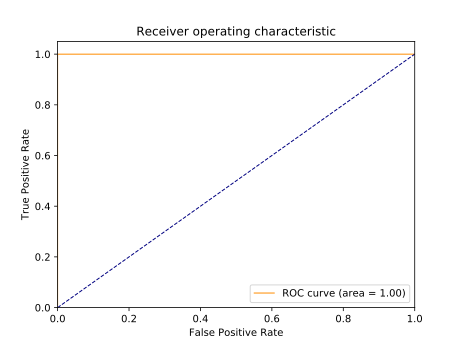
\includegraphics[width=\linewidth]{img/ruc-curve-test.svg}
		\caption{Teszt halmaz}\label{fig:roc-test}

	\end{minipage}\hfill
	\begin{minipage}[c]{0.5\linewidth}
		\includesvg[scale=0.5]{img/roc-curve-full-dataset.svg}
%		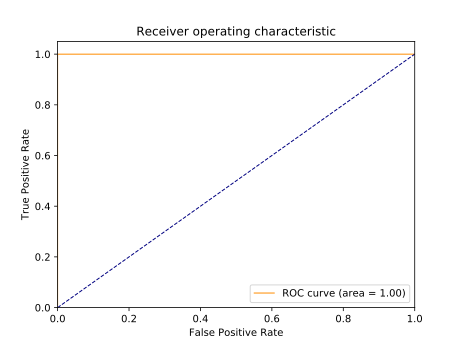
\includegraphics[width=\linewidth]{img/ruc-curve-test.svg}
		\caption{Tanító+Teszt adathalmaz}\label{fig:roc-full}
		
	\end{minipage}
	\caption{\textbf{Redukált feladat}}
	\label{fig:redukalt.feladat}
\end{figure}


Ezután ebből a hálóból kiindulva megpróbáltuk továbbtanítani, újra a teljes adathalmazon,
amelyben a kritikus minták is szerepeltek. Jól látszott a véletlen szerepe a neurális 
hálók tanításában, ugyanis csak körülbelül tizedik próbálkozásra konvergált a modell a
jó irányba, az első néhány próbálkozás a fentebb említett jelenséget produkálta: mindent 
hamisnak gondolt. Mindenesetre, végül sikerült a modellt ez alapján is betanítani, az 
eredmények pedig a \ref{fig:ujratanitott.feladat}. ábrán láthatók.


Az eredményhalmaz szeparálhatóságát, és annak korlátait a \ref{fig:histogram-ujratanitott}.
ábrán szemléltetjük, ahol egy hisztogramot láthatunk a \textit{Hamis} és az \textit{Eredeti}
halmazbeli értékek elhelyezkedéséről. Jól látható, hogy hol kell vágnunk, ha az 
első- vagy a másodfajú hibát szeretnénk csökkenteni. Ügyeljünk arra, hogy a hisztogram
logaritmikus skálát használ a jobb láthatóság kedvéért!


\begin{figure}[ht]
	
	
	\begin{minipage}[c]{0.5\linewidth}
		\includesvg[scale=0.5]{img/ruc-curve-test-ujratanitva.svg}
		%		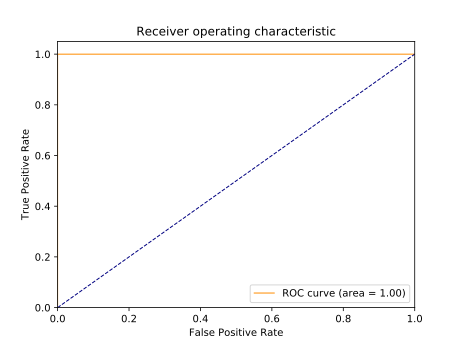
\includegraphics[width=\linewidth]{img/ruc-curve-test.svg}
		\caption{Teszt halmaz}\label{fig:roc-test}
		
	\end{minipage}\hfill
	\begin{minipage}[c]{0.5\linewidth}
		\includesvg[scale=0.5]{img/roc-curve-full-dataset-ujratanitva.svg}
		%		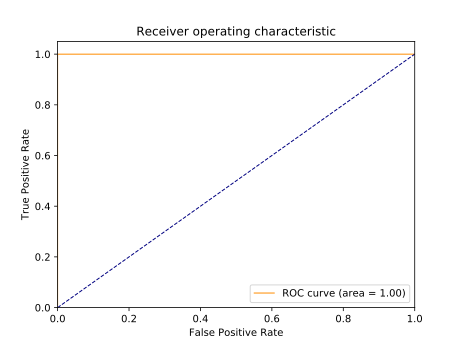
\includegraphics[width=\linewidth]{img/ruc-curve-test.svg}
		\caption{Tanító+Teszt adathalmaz}\label{fig:roc-full}
		
	\end{minipage}
	\caption{\textbf{Újratanított háló}}
	\label{fig:ujratanitott.feladat}
\end{figure}



\begin{figure}[ht]
	
	
	\begin{minipage}[c]{0.5\linewidth}
		\includesvg[scale=0.5]{img/histogram-ujratanitott-log-skala-test.svg}
		%		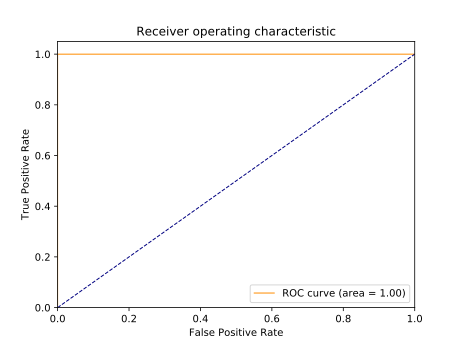
\includegraphics[width=\linewidth]{img/ruc-curve-test.svg}
		\caption{Teszt halmaz}\label{fig:hist-test}
		
	\end{minipage}\hfill
	\begin{minipage}[c]{0.5\linewidth}
		\includesvg[scale=0.5]{img/histogram-ujratanitott-log-skala-full.svg}
		%		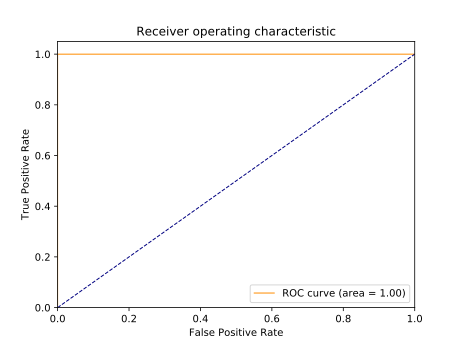
\includegraphics[width=\linewidth]{img/ruc-curve-test.svg}
		\caption{Tanító+Teszt adathalmaz}\label{fig:hist-full}
		
	\end{minipage}
	\caption{\textbf{Az újratanított háló predikciós hisztogramja}}
	\label{fig:histogram-ujratanitott}
\end{figure}


Végül nézzük az összehasonlítást az eredeti, gépi tanulást nélkülöző algoritmusokkal:


\begin{tabular}{ l l l l l }
	\underline{fájl} 			& összes minta 	& bizonytalan	& elsőfajú	& másodfajú \\
	*\texttt{bpas-verdict.csv} 	& 959 			& 0.21			& 0.1021 	& 0.0090 	\\
	*\texttt{bpas-merged.csv} 	& 496			& 0.10			& 0.1454 	& 0.0025   \\
	
	\hline
	Konvolúviós háló redukálva**& 894			& 0				& 0.02798	& 0.00972	\\
	Konvolúviós háló újratanítva& 894			& 0				& 0.05555	& 0.00900	\\
	
\end{tabular} \mbox{}


\textit{*Lásd a \ref{sec:adatok} pontot.}

\textit{**A fentiek szerint szűrt mintákon.}


Összességében azt mondhatjuk, hogy a konvolúciós háló jól teljesített, megállja a helyét 
a többi algoritmus között, az átlagos hamisítványokat nem engedi át, eredetit csak ritkán 
osztályoz félre. Ne felejtsük el, hogy több tanító példával jobb eredmény várható,
valamint elképzelhető, hogy a hiperparaméterek további optimalizálásával és háló 
szerkezetének alakításával megbízhatóbb osztályozó képességet lehet elérni. 
Továbbá ez a megoldás nem használja ki, hogy két képet készítünk, tehát ezzel még 
teljesítménynövekedést lehet elérni. További munkát igényel, hogy kidolgozzunk valamilyen
módszert arra, hogy konvolúciós hálókkal a fent említett kritikus hamisítványokat megfogjuk.
Nem elképzelhetetlen, hogy az eredeti algoritmusokkal, vagy azok SVM-el módosított változataival
párhuzamosan használjuk.




%(0.027985074626865673, 0.0097205346294045869, 0.50870099999999996)
%0.055555555555555552, 0.009009009009009028
%
%100\% lett a teszt halmazon - 120 mintából
%
%az autoencoder segített ráönni, hogy hol lett elbaszva
%nem használtuk ki hogy két képünk van
%
%
%további kutatás: további mintákkal-
%az eredményt a helyén kell kezelni - de azért bíztató
%limitáció - az offsetet nem fogta meg
%
%
%2 image merge vs sima - mi is 2 képet használtunk
%összehasonlítani a jurás eredménnyel
%
%megnézni mennyire függ a mázlitól a tanítás
%validációs hiba vs rendes hiba
%
%párhuzamosan használni a kézi elemzéssel










\newpage
\section{Konklúzió}


Bátran állíthatjuk, hogy a Gépi Tanulásnak van helye az eredetiség vizsgálat témakörében.
Igaz, a módszer még nem elég kifinomult ahhoz, hogy azonnal ipari környezetben használjuk,
azt mindenképpen bizonyítottunk, hogy ígéretes kutatási terület, és lehet jövője éles 
helyzetekben is.


Az SVM, vagy akár egyéb gépi tanulásra alapuló algoritmus tökéletesen illeszkedik
a döntéshozás munkamenetébe, és kétség sem fér a hasznosságához. A kockázata sem 
túl nagy, hiszen a működési mechanizmusa hasonlít ahhoz amit egy programozó kézzel írna.
Az SVM jó tulajdonsága a magyarázó képesség. Egy neuronhálóval ellentétben ha rátekintünk
a paraméterekre meg tudjuk mondani, hogy egy adott döntést hozott, és ha ezzel nem vagyunk 
elégedettek tudjuk hova kell nyúlni.


Egy konvolúciós háló sokkal erőforrás-igényesebb, és egy teljesen más megközelítés,
amely még csak nem is hasonlít az eddig használt algoritmusokhoz, ezért óvatosan kell 
kezelni. Hátránya, hogy ha valami nem működik nehéz kinyomozni, ahogy fentebb említettük
kifejezetten rossz a magyarázóképessége. Problémát okozhat a használata kis erőforrással 
rendelkező rendszerekben: GPU nélkül neki sem érdemes látni. A rejtett rétegek súlyai is 
meglehetősen sok helyet foglalnak, jelen pillanatban 120 megabájt körül van, de ha tegyük
fel egy telefon makrolencsével készült teljes képét ki szeretnénk elemezni, 
amelyek csúcskategóriás készülékeknél bőven 10 megapixel felett van, akkor hatalmasra 
nőhet a belső reprezentáció. Véleményem szerint még több évnyi munka kell ahhoz, hogy 
ebből egy megbízható alkalmazás legyen, ami minden körülmények között meg tud 
különböztetni egy hamis pénzt egy eredetitől.


\subsection{További feladatok}

Amennyiben ebből használható alkalmazást szeretnénk készíteni át kell ültetnünk mobil 
platformra. Nem kétséges, hogy a mai mobil GPU-k már hatékonyan fognak megbirkózni a
feladattal. Ne felejtsük el, hogy bár egy neuronhálót betanítani idő- és erőforrás-igényes,
használni már jóval egyszerűbb, feltéve, hogy a modellt egy az egyben beleépítjük a használó
alkalmazásba.


A dolgozathoz a projekt \texttt{pythonban} készült. Ez egy roppant flexibilis nyelv, és
kiváló prototípus készítéshez, de tekintve, hogy egy szkriptnyelv, a hibakezelés a 
típusosság hiányában sokkal nehezebb. Ezért célszerűnek látom az éles környezetben 
való használathoz egy fordítóval rendelkező, biztonságos, de mégis hatékony nyelven 
való megvalósítást, erre \texttt{C++}-t javaslok. Ehhez létezik kiegészítő könyvtár,
amivel a \texttt{Keras}\cite{keras} által készített modellt használni tudjuk. Az ehhez szükséges
\texttt{Tensorflow}\cite{tensorflow} csomag szintén elérhető.


Preferenciáktól függő feladat egy \textit{Bizonytalan} intervallum bevezetése minden
projekthez, amelyhez szükségünk van egy maximálisan eltűrt első- és másodfajú hibarátára.

\subsection{Kutatási területek}

A képek normalizálása során felmerült, hogy bár a pozicionáló koordináták rendelkezésünkre 
álltak, a konvolúciós hálók alkalmasak lehetne ezek hatékony megtalálására.


Ahogy az eredményeknél elemeztük, kutatást igényel bizonyos trükkös képek elemzése,
ez még a jövő feladata.

%
%további feladatok:
%
%például mobilra átültetni
%dunno bevezetése
%emberi programozási nyelv - ez csak prototípus annak minden bajával
%
%
%lehetne majd pozicionálásra is megpróbálni
%
%
%kis kikockázás
%
%batch, eposz
%dropout, normalizálás, balancing, augmentation
%loss/accuracy - roc görbe "siker mérése"
%test/val/train
%early stopping
%MERGED images??? dunno?


\newpage
\section{Útmutató a kódhoz}

akár az argparse is mehet
numpy
keras
sklearn
tensorflow
cuda
cuda nn
winpython 3.6
hyperopt
matplotlib
opencv
visual studio - working dir
csomagokhoz->pip

\newpage
\begin{thebibliography}{9}
	\bibitem{adam} 
	Diederik P. Kingma, Jimmy Ba:
	Adam: A Method for Stochastic Optimization
	arXiv:1412.6980v9 [cs.LG]
	
	
	\bibitem{numpy} 
	\url{http://www.numpy.org}
	

	\bibitem{sklearn} 
	\url{http://scikit-learn.org/stable/modules/generated/sklearn.svm.SVC.html}
	
	\bibitem{svm.c} 
	\url{http://scikit-learn.org/stable/auto_examples/svm/plot_rbf_parameters.html}
	
	\bibitem{sklearn.regularization} 
	\url{http://scikit-learn.org/stable/auto_examples/svm/plot_svm_scale_c.html}
	
	\bibitem{hyperopt} 
	\url{https://github.com/hyperopt/hyperopt}
	
	\bibitem{keras} 
	\url{https://keras.io/}
	
	\bibitem{tensorflow} 
	\url{https://www.tensorflow.org/}

	\bibitem{opencv} 
	\url{https://opencv.org/}
	
\end{thebibliography}




%I think we did a pretty good\textsuperscript{\textit{job}}so far



